% Prepared by Karl Ecklund September 2002
% Questions, Improvements, Comments to kme and CLEOAC
%
% LATEX 2e Template for CLEO Papers
% YOU MUST USE REVTEX4 and latex 2e
%
% Checklist for Paper Drafts:
% ---------------------------
% 0) Use appropriate \documetclass line as indicated below
% 1) Draft Number: Use latest CBX number, append A for the first vote
%                                (B,C,... for subsequent if any votes)
% 2) Don't use CLNS or CLEO numbers - this happens after your vote.
% 3) Title; use \\ to break title over several lines.
% 4) Abstract
% 5) For the Author list use CLEO Collaboration only
% 6) Body
% 
% Checklist for Journal Submissions:
% ----------------------------------
% 0) Use appropriate \documetclass line as indicated below
%    - For CLNS, hep-ex, preprints, conf. paper use CLNS version
%    - For PRL submission use PRL version
%    - For PRD submission use PRD version 
%      AND use \author{(CLEO Collaboration)} instead of \collaboration{CLEO}
%      SEE PRD_SPECIAL_CHANGEME in author list during step 5 below
% 1) CLEO paper number (from CLEOAC)
% 2) CLNS preprint number (from CLEOAC)
% 3) Title; use \\ to break title over several lines.
% 4) Abstract
% 5) Author list (from CLEOAC)
% 6) PACS codes
% 7) Body
% 8) Add acknowledgments
% 9) Hardcode the \date when ready to submit to journal and hep-ex.
%
% Checklist for Conference Papers:
% --------------------------------
% 0) Use appropriate \documetclass line as indicated below
%    - For conf. paper use CLNS version
% 1) CLEO conference paper number (from CLEOAC) (don't use CLNS)
% 2) Title; use \\ to break title over several lines.
% 3) To \thanks after title, add appropriate conference info.
% 4) Abstract
% 5) Author list (from CLEOAC)
% 6) Body
% 7) Add acknowledgments
% 8) Hardcode the \date when ready to submit to conference and hep-ex.
% 
% KNOWN PROBLEMS with template and REVTEX4
% - can't have \collaboration in PRD style grouped author list
%   Using \author{(CLEO Collaboration)} instead
% - can't make abstract appear before full author list ala CLNS notes
%   Abandoning this as the format for CLNS.

%%%%%%%%%%%%%%%%%%%%%%%%%%%%%%%%%%%%%%%%%%%%%%%%%%%%%%%%%%%%%%%%%%%%%%
% Select one of the \documentclass lines below for your paper
%%%%%%%%%%%%%%%%%%%%%%%%%%%%%%%%%%%%%%%%%%%%%%%%%%%%%%%%%%%%%%%%%%%%%%
%%%%%%%%%%%%%% Use for CLNS preprint (hep-ex) and Paper Drafts
%\documentclass[aps,prd,preprint,superscriptaddress,tightenlines,nofootinbib]{revtex4}

%%%%%%%%%%%%%% Use for PRL
\documentclass[aps,prl,twocolumn,superscriptaddress,showpacs]{revtex4}

%%%%%%%%%%%%%% Use for PRD
%\documentclass[aps,prd,twocolumn,nofootinbib,showpacs]{revtex4}

\usepackage{graphicx}% Include figure files
\usepackage{dcolumn}% Align table columns on decimal point
\usepackage{bm}% bold math

\begin{document}

%\preprint line(s) will be ignored for PRL/PRD
%\preprint{CLEO Draft YY-NNA} % For paper draft CBX YY-NN -> Draft YY-NNA
%\preprint{CLEO CONF YY-NN}   % For conference papers
%\preprint{ICHEP ABSnnn}      % For conference papers
\preprint{CLNS YY/NNNN}       % for CLNS notes
\preprint{CLEO YY-NN}         % for CLNS notes

\title{Di-electron Widths of the Upsilon(1S,2S,3S) Resonances}
% for conference papers (ask CLEOAC for appropriate text)
%\thanks{Submitted to the 31$^{\rm st}$ International Conference on High Energy
%Physics, July 2002, Amsterdam}

%-------- INSERT HERE ------------
% Your author list goes here  REMOVE EVERYTHING to END INSERT and
% replace with your authorlist (ask cleoac).

\author{J.~Pivarski}
\author{J.R.~Patterson}
\author{K.~Berkelman}
\affiliation{F.~R.~Newman Laboratory for Elementary-Particle Physics,
Ithaca, New York 14853-8001}

%\author{(CLEO Collaboration)}     %FOR PRD_SPECIAL_CHANGEME
\collaboration{CLEO Collaboration} %FOR PRL and CLNS (superscriptaddress)
\noaffiliation

%-------- END INSERT ------------

%please hard code the date when you have a final draft and submit to CLEOAC
\date{\today}

\newcommand{\gee}{$\Gamma_{ee}$}
\newcommand{\ups}{$\Upsilon$}
\newcommand{\us}{$\Upsilon(1S)$}
\newcommand{\uss}{$\Upsilon(2S)$}
\newcommand{\usss}{$\Upsilon(3S)$}
\newcommand{\ee}{$e^+e^-$}
\newcommand{\mm}{$\mu^+\mu^-$}
\newcommand{\tautau}{$\tau^+\tau^-$}
\newcommand{\ellell}{$\ell^+\ell^-$}
\newcommand{\pipi}{$\pi^+\pi^-$}
\newcommand{\PM}{$\pm$}
\newcommand{\inv}{$^{-1}$}
\newcommand{\bmm}{${\mathcal B}_{\mu\mu}$}
\newcommand{\btt}{${\mathcal B}_{\tau\tau}$}
\newcommand{\geehadtot}{\Gamma_{ee}\Gamma_{\mbox{\scriptsize had}}/\Gamma_{\mbox{\scriptsize tot}}}
\newcommand{\pvis}{P_{\mbox{\scriptsize vis}}}
\newcommand{\ppass}{P_{\mbox{\scriptsize pass given vis}}}
\newcommand{\ehtrig}{\epsilon_{\mbox{\scriptsize htrig}}}
\newcommand{\ecuts}{\epsilon_{\mbox{\scriptsize cuts}}}

\begin{abstract} 
We have determined the di-electron widths of the \us, \uss, and \usss\
to be 1.360 \PM\ 0.004 {\it (stat)} \PM\ 0.022 {\it (syst)} keV, 0.620
\PM\ 0.004 \PM\ 0.011 keV, and 0.447 \PM\ 0.004 \PM\ 0.007 keV,
respectively.  To measure these widths to their 2\% precisions, the
Cornell Electron Storage Ring scanned beam energy across production
cross-section lineshapes of the three resonances in \ee\ collisions,
providing the CLEO detector with a total of 0.61 fb\inv\ of lineshape
data and 0.76 fb\inv\ below resonance for background subtraction.
These measurements are a precise check on QCD calculations,
particularly lattice QCD.
\end{abstract}

\pacs{13.20.He}
\maketitle

Recent progress in lattice QCD has renewed interest in the \ee\ decay
rate (di-electon width, or \gee) of the $b\bar{b}$ bound states \us,
\uss, and \usss.  Theorists are now calculating \gee\ on the lattice
without the quenched approximation (that is, without ignoring vacuum
polarization) \cite{latgee} as a demonstration of the improved
algorithms.  But the experimental resolution is currently inadequate
to provide a tight constraint: \gee\ of the \us, \uss, and \usss\ are
known to 2.2\%, 4.2\%, and 9.4\% of themselves, respectively
\cite{pdg}.  We present a high-precision measurement of \gee\ for all
three narrow \ups\ resonances.

This test of lattice QCD is especially interesting because it will
check lattice calculations of the $B$ meson decay constant $f_B$
\cite{latfb}, which, if trusted to high accuracy, would dramatically
improve our knowledge of the CKM matrix element $V_{td}$.  Both are
calcuations of the $q\bar{q}$ spatial wavefunction at the origin,
$b\bar{b}$ in the case of \gee, and $b\bar{d}$ in the case of $f_B$.
It compliments the CLEO-c measurement of $f_D$ \cite{fd}, which tests
calculations of $c\bar{d}$.

This measurement also benefits potential model fits, since we
significantly constrain $\Gamma_{ee}(\Upsilon(3S))$ over the previous
measurement.

Our measurement of \gee\ follows the method of \cite{pdg}: we measure
the production cross-section of the time-reversed process, $e^+e^- \to
\Upsilon$, integrated over incident \ee\ energies.  Then,
\begin{equation}
\label{eqn:gee}
\Gamma_{ee} = \frac{{M_\Upsilon}^2}{6\pi^2}\int \sigma(e^+e^- \to
\Upsilon) \, dE \mbox{.}
\end{equation}
We correct the production cross-section for initial state radiation,
which means that we quote only the non-radiative \gee.  We do not,
however, make any correction to remove vacuum polarization.  Since
this measurement of decay rate is independent of the branching
fraction ${\mathcal B}_{ee}$, we will also determine the \ups\ full
width assuming ${\mathcal B}_{ee}$ = \bmm\ so that we can take
advantage of \bmm, the best-measured leptonic branching fraction
\cite{istvan}.

To measure \gee, the Cornell Electron Storage Ring, a symmetric \ee\
collider, scanned center-of-mass energies in the vicinity of the \us,
\uss, and \usss\ and the CLEO-III detector collected the \ups\ decay
products to determine the cross-section at each beam energy.  The
integral in Equation \ref{eqn:gee} is then extracted by a fit to this
resonance lineshape.  The fit includes beam energy spread, initial
state radiation, backgrounds, and interference between \ups\ and
continuum final states.  The 11 (6, 7) \us\ (\uss, \usss) scans
consist of 0.10 (0.06, 0.10) fb\inv, with 0.18 (0.44, 0.16) fb\inv\ of
continuum data taken 20 MeV below the resonance to constrain
backgrounds.

The CLEO-III detector is a nearly 4$\pi$ tracking volume surrounded by
a CsI crystal calorimeter \cite{cleoiii}.  Charged tracks are
reconstructed in a 47-layer wire drift chamber and 4-layer silicon
strip detector, and their momenta are inferred from their radii of
curvature in a 1.5 T magnetic field.  The calorimeter forms a
cylindrical barrel around the tracking volume, reaching angles
$\theta$ with respect to the beam axis of $|\cos\theta|$ $<$ 0.85,
with endcaps extending this range to $|\cos\theta|$ $<$ 0.98.
Electron and photon showers have a resolution of $x$ MeV at beam
energy (5 GeV).

The \ups\ mesons are produced at rest and decay into leptonic final
states $e^+e^-$, $\mu^+\mu^-$, and $\tau^+\tau^-$, or into hadrons
with a typical multiplicity of 10 through $ggg$, $gg\gamma$, and
$q\bar{q}$.  The \uss\ and \usss\ can also decay spectroscopically
into other $b\bar{b}$ resonances such as $\chi_{b0,1,2}(nP)$, \us, and
\uss.  The leptonic final states together account for only 7\% of the
decays but are difficult to distinguish from background, so we select
for hadrons, fit the hadronic cross-section, and correct for the
missing leptonic modes by dividing by $(1 - 3{\mathcal B}_{\mu\mu})$.
We will also quote $\geehadtot$, which does not include this
correction.

Bhabha scattering ($e^+e^- \to e^+e^-$) is our largest background.  We
suppress these events by requiring the greatest track momentum to be
less than 80\% of the beam energy, shown in Figure \ref{fig:cuts}-a,
which reduces the Bhabha background to approximately the same
magnitude as the hadronic continuum ($e^+e^- \to q\bar{q}$).  Most
continuum processes are accounted for by including a $1/s$ term in the
lineshape fit.

\begin{figure}
  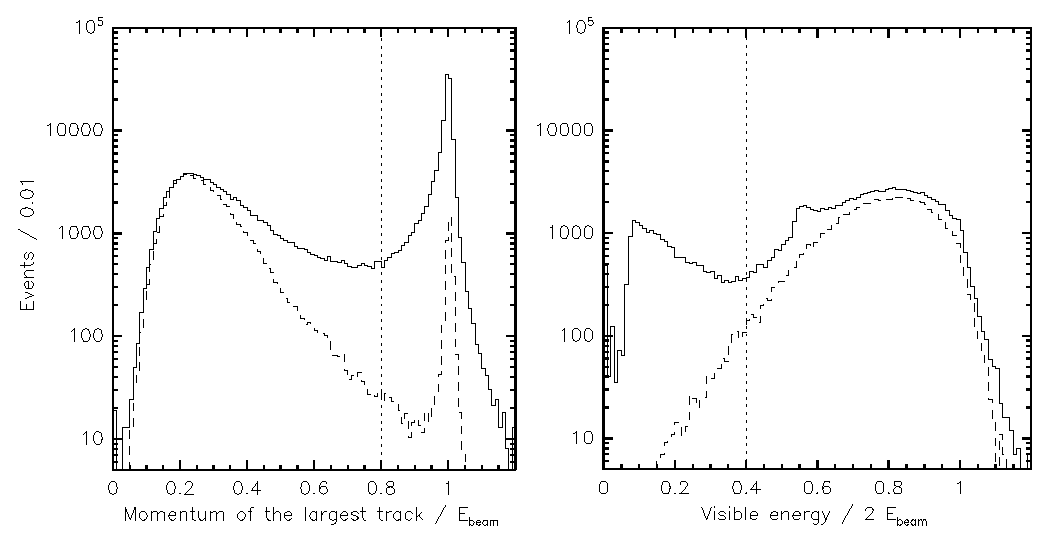
\includegraphics[width=\linewidth]{cuts}
  \caption{\label{fig:cuts} Two of the four hadronic selection
  criteria: a) the greatest track momentum must be less than 80\% of
  the beam energy, and b) the visible energy in the event must be more
  than 40\% of the center-of-mass energy.  Solid histograms are data,
  dashed are simulated \ups\ decays with the same normalization.  Note
  the log scale.}
\end{figure}

Two-photon fusion events ($e^+e^- \to e^+e^- X$) contribute a
non-$1/s$ background, so we suppress these by requiring the total
visible energy (energy sum of all charged tracks and neutral showers)
to be more than 40\% of the center-of-mass energy (twice the beam
energy), shown in Figure \ref{fig:cuts}-b.  A small $\log s$ term (8\%
of continuum below \us) and $1/(\sqrt{s}-M_\Upsilon)$ terms
(representing radiative returns to lower \ups\ resonances, about 0.5\%
of continuum) are also added to the fit function.  Because the
continuum measurement is only 20 MeV below the resonance, the
different functional forms affect the background estimation at the
peak by less than 0.04\%.

Cosmic rays and beam-gas (collisions between a beam electron and a gas
atom inside the beampipe) are suppressed by requiring charged tracks
to point toward the collision point.  At least one track must pass
within 5 mm of the beam axis and the vertex reconstructed from all
primary tracks must be within 7.5 cm of the collision point along the
beam axis.  These two requirements have 99.9\% and 99.4\% efficiencies
for \ups\ decays, respectively, and reduce the backgrounds to less
than 1\% of the continuum background.  We determine the contamination
at each energy using special single-beam and no-beam data runs
normalized using events with a solitary large impact parameter track
(for cosmic rays) or events with vertices along the beam axis but far
from the collision point (for beam gas).

All background estimations are presented in Figure
\ref{fig:backgrounds}.

\begin{figure}
  \includegraphics[width=\linewidth]{backgrounds}
  \caption{\label{fig:backgrounds} Hadronic events divided by
  luminosity versus energy in log scale, showing all background
  components.  The fit function includes a $1/s$ term to account for
  most continuum processes and non-$1/s$ corrections from two-photon
  fusion and radiative returns to lower \ups\ resonances.  Cosmic rays
  and beam-gas are explicitly subtracted.}
\end{figure}

These four requirements eliminate $\Upsilon \to e^+e^-$ and $\Upsilon
\to \mu^+\mu^-$ modes, and they pass only 57\% of $\Upsilon \to
\tau^+\tau^-$, as determined by a GEANT-based Monte Carlo simulation
\cite{mc}.  We therefore include an $\Upsilon \to \tau^+\tau^-$
background term in the fit function.

A small fraction of hadronic \ups\ decays fail our event selection
criteria, so we must correct for this inefficiency.  Instead of
estimating it with a Monte Carlo simulation, which would introduce
dependence on the hadronization model and the assumption that all
\ups\ decays are known, we use a data-based approach.  We select
$\Upsilon(2S) \to \pi^+\pi^- \, \Upsilon(1S)$ to study \us\ decays
tagged by the \pipi.  If the \pipi\ were sufficient to satisfy the
trigger, the \us\ decays would be completely unbiased: the efficiency
would be the ratio of \us\ events satisfying our selection criteria
(excluding the \pipi\ tracks) to all \us\ events.

To apply the above procedure, we use a 1.3 fb\inv\ sample of \uss\
decays.  We select events accepted by our two-track trigger containing
a pair of tracks consistent with recoil from an \us.  We additionally
require both tracks to have more than 150 MeV of momentum transverse
to the beam axis, so that these two tracks alone satisfy the two-track
trigger with 99.93\% probability.  The mass of the system recoiling
against these \pipi\ candidates has a prominent peak at the \us\ mass
as shown in Figure \ref{fig:cascades}-a and a background from
miscombinations that is linear in mass.  If we apply our event
selection and form a ratio as described in the preceeding paragraph,
we can only determine the hadronic efficiency to 3\% of itself,
because the two-track trigger is prescaled by a factor of 20.
Therefore, we measure the efficiency in two stages: we use the
two-track trigger to determine the efficiency of an unprescaled but
more restrictive hadronic trigger ($\ehtrig$), and then use the full
statistics from that trigger to determine our selection efficiency,
given events that have passed the hadronic trigger ($\ecuts$).  Our
selection efficiency for \us\ events is the product of these two
factors: $\ehtrig$ corrects for the small bias introduced by using the
hadronic trigger to determine $\ecuts$.  Counting the events that fail
the hadronic trigger, shown in Figure \ref{fig:cascades}-b, we find $1
- \ehtrig$ = (0.41 $^{+0.45}_{-0.29}$)\%, where we have corrected for
the presence of leptonic modes in the \us\ sample.  To determine
$\ecuts$, we count events passing the hadronic trigger, with and
without our event selection criteria.  We then correct for leptonic
modes, the tiny boost of the \us, and track confusion from the \pipi.
The combined efficiency of our trigger and event selection is (97.93
$^{+0.44}_{-0.56}$)\%.

\begin{figure}
  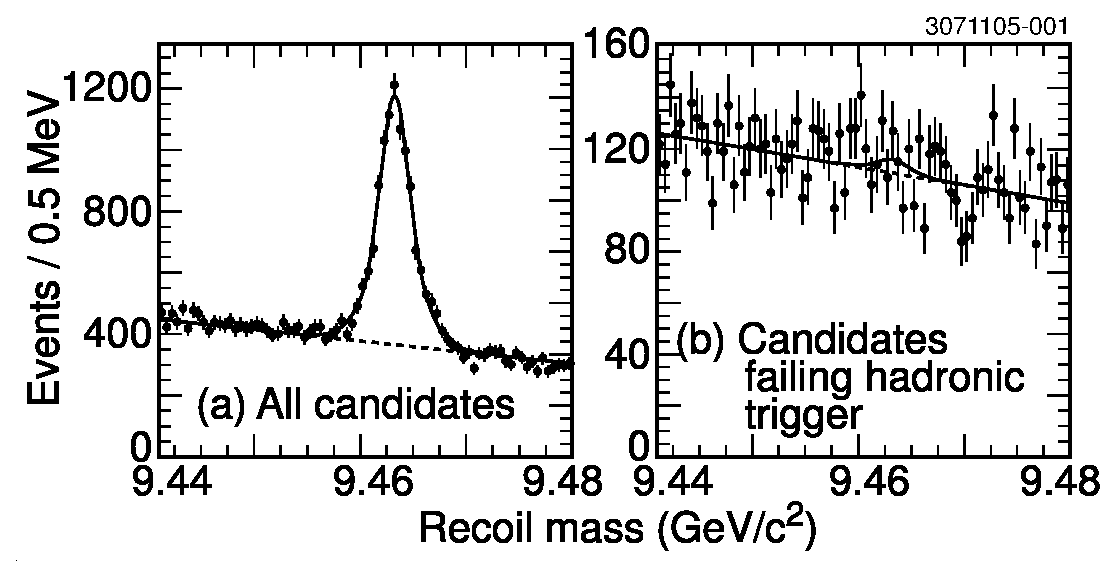
\includegraphics[width=\linewidth]{cascades}
  \caption{\label{fig:cascades} Recoil mass of $\pi^+\pi^-$ in the
  hadronic efficiency study, a) for all events from the two-track
  trigger and b) for those which fail the hadronic trigger.  The solid
  line is a fit to a double Gaussian with a linear background
  (dashed).  In (b), the mean, sigmas, and area ratio of the double
  Gaussian are not allowed to float.}
\end{figure}

To find the \uss\ and \usss\ efficiencies, we correct the \us\
efficiency for energy dependence and decay modes specific to these
excited states, using simulations.  Energy dependence in $ggg$,
$gg\gamma$, and $q\bar{q}$ and most spectroscopic decays affect the
\uss\ and \usss\ efficiencies negligibly (a 0.2\% downward
correction), but spectroscopic decays to a lower \ups\ which then
decays to $e^+e^-$ or $\mu^+\mu^-$ have negligible efficiency.  We
measure the branching fractions of these $X\ell^+\ell^-$ decays to be
(1.58 \PM\ 0.16)\% and (1.34 \PM\ 0.13)\%, respectively.  The hadronic
efficiencies of the \uss\ and \usss\ are therefore (96.18
$^{+0.44}_{-0.56}$ \PM\ 0.15)\% and (96.41 $^{+0.44}_{-0.56}$ \PM\
0.13)\%, respectively.

To determine the integrated luminosity of each energy point, we select
Bhabhas by requiring two or more tracks with momenta between 50\% and
110\% of the beam energy.  The energy sum of the two tracks with greatest
momentum plus the energy of associated bremsstrahlung photons must be
more than 90\% of the center-of-mass energy, the larger (smaller)
$\cos \theta$ must be less than 0.766 (0.707) where $\theta$ is the
angle between the track and the beam axis, and the larger (smaller)
$E/p$ must be greater than 0.8 (0.5) where $E$ is the shower energy
of the electron and $p$ is its track momentum.  Contamination from
$\Upsilon \to e^+e^-$ is about 3\% and is readily calculated given
\bmm\ once we have done our \ups\ lineshape fit.  Our subtraction
includes interference between $\Upsilon \to e^+e^-$ and Bhabhas.

We normalized the Bhabha luminosity using the method of \cite{oldlumi}
with the {\textsc Babayaga} event generator \cite{babayaga}.  We also
normalized $e^+e^- \to \mu^+\mu^-$ and $e^+e^- \to \gamma\gamma$ with
{\textsc Babayaga}.  The systematic uncertainties in the luminosity
for Bhabhas, $\mu^+\mu^-$, and $\gamma\gamma$ are 1.6\%, 1.6\%, and
1.8\%, respectively, dominated by track finding and resonance
interference for the leptonic final states and photon finding and cut
variation for $\gamma\gamma$.  The three final states give consistent
results off-resonance, where \ups\ contamination is negligible.  The
RMS scatter of the three measurements is 1.3\%, which we take as the
systematic uncertainty in the normalization, for which we use the
weighted mean.  Bhabha and $\gamma\gamma$ luminosity, normalized to
the same value off-resonance, were found to deviate by less than 0.8\%
(0.5\%, 0.7\%) when extrapolated to the \us\ (\uss, \usss) peak, so we
add this as a systematic uncertainty in the consistency of the
luminosity through each scan.

If the beam energy measurement drifts during a scan, it may widen or
narrow the fitted peak.  The beam energy is measured by an NMR probe
in a test dipole magnet in series with the beam magnets, with
corrections for RF frequency shifts, steering and focusing magnets,
and electrostatic electron-positron separators.  To limit our
sensitivity to drifts in this measurement, we limit scans to 48 hours
and alternate measurements above and below the peak.  While repeated
scans indicate that the calibration of the 5 GeV beam energy drifts as
much as 0.3 MeV between scans, repeated cross-section measurements at
the same energy during a scan indicate that the beam energy
calibration drifts by less than 0.04 MeV within a scan (68\% C.L.),
which translates to a 0.2\% uncertainty in \gee.

The fit function consists of a Breit-Wigner resonance (including
interference between continuum $q\bar{q}$ and $\Upsilon \to
q\bar{q}$), convoluted with a Gaussian beam energy spread and
radiative corrections ($e^+e^- \to \gamma \Upsilon$, a high-energy
tail) calculated by Kureav and Fadin \cite{kf}.  As explained above,
$1/s$, non-$1/s$, and $\Upsilon \to \tau^+\tau^-$ backgrounds are
included as additional terms (with continuum-resonance interference
for $\tau^+\tau^-$).  Each of the three independent fits (one for each
resonance) combines data from all scans, with free parameters for
\gee, the background normalization, and, to remove sensitivity to beam
energy shifts between scans, the peak energy of each scan.  In
addition, we fit for the beam energy spread of groups of scans with
common horizontal steerings, but allow shifts when the steerings
change, since they affect beam energy spread at the level of 1\% of
itself.  The largest systematic uncertainties in the shape of the fit
function come from the normalization of the radiative corrections and
$\tau^+\tau^-$ interference: these lead to a 0.1\% uncertainty in
\gee.

Fit results are plotted in Figure \ref{fig:fits}.  The reduced
$\chi^2$ for \us, \uss, and \usss\ are $240/(203-16) = 1.3$,
$107.2/(75-9) = 1.6$, and $155/(175-16) = 0.97$, respectively.  Pull
distributions versus energy and versus date do not show any obvious
trends, and the width of a Gaussian fit to each pull distribution
yields a sigma which is the square root of the reduced $\chi^2$.
Therefore, we take the large reduced $\chi^2$ values as an indication
of a small cross-section instability which has not been accounted for,
and add $\sqrt{\chi^2/ndf - 1^2} \sigma_{\mbox{\scriptsize stat}}$ as
a systematic uncertainty, where $\sigma_{\mbox{\scriptsize stat}}$ is
the statisitcal uncertainty, for each resonance.

\begin{figure}
  \includegraphics[width=\linewidth]{fits}
  \caption{\label{fig:fits} Fits to \us, \uss, and \usss\ hadronic
  cross-section versus center-of-mass energy lineshapes, left to
  right.  Points are data, corrected for beam energy shifts between
  scans, the solid line is the fit, the dashed line is sum of all
  backgrounds, and the insets show high-energy measurements, 100 MeV,
  60 MeV, and 45 MeV above the peaks, left to right.  The continuum
  background includes 3.4 nb (9.44 GeV)$^2$/$s$ of radiative Bhabhas.}
\end{figure}

All uncertainties in \gee\ are listed in Table \ref{tab:unc}.

\begin{table}
  \renewcommand{\arraystretch}{1.25}
  \begin{tabular}{l c c c}
    \hline\hline Contribution to \gee & \hspace{0 cm}\us\hspace{0 cm} & \hspace{0 cm}\uss\hspace{0 cm} & \hspace{0 cm}\usss\hspace{0 cm} \\\hline
    Statistical                                    & 0.3\% 	      & 0.7\%  & 1.0\% \\
    $(1 - 3\mathcal{B}_{\mu\mu})$                  & 0.2\% 	      & 0.2\%  & 0.3\% \\
    Hadronic efficiency                            & $\longleftarrow$ & 0.5\%  & $\longrightarrow$ \\
    Hadronic efficiency ($Xe^+e^-$, $X\mu^+\mu^-$) & 0                & 0.15\% & 0.13\% \\
    Luminosity normalization                       & $\longleftarrow$ & 1.3\%  & $\longrightarrow$ \\
    Luminosity consistency                         & 0.8\%  	      & 0.5\%  & 0.7\% \\
    Beam energy measurement drift                  & 0.2\%  	      & 0.2\%  & 0.2\% \\
    Shape of the fit function                      & 0.05\% 	      & 0.05\% & 0.05\% \\
    Cross-section instability                      & 0.2\%  	      & 0.9\%  & 0 \\\hline
    Fractional uncertainty                         & 1.7\%    	      & 1.9\%  & 1.9\% \\\hline\hline
  \end{tabular}
  \caption{\label{tab:unc} All uncertainties in \gee\ measurements in
  the order in which they were discussed in the text.  Uncertainties
  that are common to all resonances are indicated with arrows.}
\end{table}

\begin{table}
  \renewcommand{\arraystretch}{1.25}
  \begin{tabular}{c c c}
    \hline\hline $\Gamma_{ee}(1S)$ & \hspace{1.5 cm} & (1.360 \PM\ 0.004 \PM\ 0.022) keV \\
    $\Gamma_{ee}(2S)$ & & (0.620 \PM\ 0.004 \PM\ 0.011) keV \\
    $\Gamma_{ee}(3S)$ & & (0.447 \PM\ 0.004 \PM\ 0.007) keV \\\hline
    $\Gamma_{ee}(2S)/\Gamma_{ee}(1S)$ & & (0.456 \PM\ 0.005 \PM\ 0.006) \\
    $\Gamma_{ee}(3S)/\Gamma_{ee}(1S)$ & & (0.329 \PM\ 0.006 \PM\ 0.004) \\
    $\Gamma_{ee}(3S)/\Gamma_{ee}(2S)$ & & (0.721 \PM\ 0.006 \PM\ 0.009) \\\hline
    $\geehadtot(1S)$ & & (1.257 \PM\ 0.004 \PM\ 0.020) keV \\
    $\geehadtot(2S)$ & & (0.620 \PM\ 0.004 \PM\ 0.011) keV \\
    $\geehadtot(3S)$ & & (0.415 \PM\ 0.004 \PM\ 0.007) keV \\\hline\hline
  \end{tabular}
  \caption{\label{tab:results} The values of \gee\ for the three
  resonances, ratios of the three resonances, and $\geehadtot$
  (calculated without assuming Lepton Universality).  The first
  uncertainty is statistical (hadronic event and Bhabha counting) and
  the second is systematic (everything else).}
\end{table}

Values of \gee, along with their ratios and $\geehadtot$, are listed
in Table \ref{tab:results}.  Our measurements are consistent with, but
more precise than, the PDG world averages \cite{pdg}, provide the
first precision measurement of $\Gamma_{ee}(3S)$, and largely share
systematic uncertainties, making the ratios even more precise.  We
calculate $\geehadtot$ using ${\mathcal B}_{\tau\tau}$ \cite{jean} to
normalize the $\tau^+\tau^-$ background, thereby avoiding assumptions
of Lepton Universality.  Combining \gee\ with \bmm\ (\cite{istvan}),
we obtain new values of the \ups\ full widths: 54.6 \PM\ 1.9 keV, 30.6
\PM\ 1.4 keV, and 18.7 \PM\ 1.0 keV, respectively.

We gratefully acknowledge the effort of the CESR staff 
in providing us with excellent luminosity and running conditions.
This work was supported by 
the A.P.~Sloan Foundation,
the National Science Foundation,
and the U.S. Department of Energy.

\begin{thebibliography}{99}

\bibitem{cleoiii}
G. Viehhauser {\it CLEO III Operation},
Nucl. Instrum. Methods A {\bf 462}, 146 (2001).

\bibitem{oldlumi}
G.D. Crawford {\it et al.} (CLEO Collaboration), Nucl. Instrum. Methods Phys. Res., Sect A {\bf 345}, 429 (1994).

\bibitem{babayaga}
C.M.~Carloni~Calame {\sl et al.},
Nucl. Phys. Proc. Suppl. B {\bf 131}, 48 (2004).

\end{thebibliography}
\end{document}
